%\documentclass{article}
%
%\usepackage{fancyhdr}
%\usepackage{extramarks}
%\usepackage{amsmath}
%\usepackage{amsthm}
%\usepackage{amsfonts}
%\usepackage{tikz}
%\usepackage{enumerate}
%\usepackage{graphicx}
%\graphicspath{ {images/} }
%\usepackage[plain]{algorithm}
%\usepackage{algpseudocode}
%\usepackage[document]{ragged2e}
%\usepackage{textcomp}
%\usepackage{color}   %May be necessary if you want to color links
%\usepackage{import}
%\usepackage{hyperref}
%\hypersetup{
%    colorlinks=true, %set true if you want colored links
%    linktoc=all,     %set to all if you want both sections and subsections linked
%    linkcolor=black,  %choose some color if you want links to stand out
%}
%
%\usetikzlibrary{automata,positioning}
%
%%
%% Basic Document Settings
%%
%
%\topmargin=-0.45in
%\evensidemargin=0in
%\oddsidemargin=0in
%\textwidth=6.5in
%\textheight=9.0in
%\headsep=0.25in
%\setlength{\parskip}{1em}
%
%\linespread{1.1}
%
%\pagestyle{fancy}
%\lhead{\hmwkAuthorName}
%\lfoot{\lastxmark}
%\cfoot{\thepage}
%
%\renewcommand\headrulewidth{0.4pt}
%\renewcommand\footrulewidth{0.4pt}
%
%\setlength\parindent{0pt}
%
%
%\newcommand{\hmwkTitle}{Math Review Notes---Calculus}
%\newcommand{\hmwkAuthorName}{\textbf{G. Faletto} }
%
%%
%% Title Page
%%
%
%\title{
%    \vspace{2in}
%    \textmd{\textbf{ \hmwkTitle}}\\
%}
%
%\author{Gregory Faletto}
%\date{}
%
%\renewcommand{\part}[1]{\textbf{\large Part \Alph{partCounter}}\stepcounter{partCounter}\\}
%
%%
%% Various Helper Commands
%%
%
%% Useful for algorithms
%\newcommand{\alg}[1]{\textsc{\bfseries \footnotesize #1}}
%
%% For derivatives
%\newcommand{\deriv}[2]{\frac{\mathrm{d} #1}{\mathrm{d} #2}}
%
%% For partial derivatives
%\newcommand{\pderiv}[2]{\frac{\partial #1}{\partial #2}}
%
%% Integral dx
%\newcommand{\dx}{\mathrm{d}x}
%
%% Alias for the Solution section header
%\newcommand{\solution}{\textbf{\large Solution}}
%
%% Probability commands: Expectation, Variance, Covariance, Bias
%\newcommand{\E}{\mathbb{E}}
%\newcommand{\Var}{\mathrm{Var}}
%\newcommand{\Cov}{\mathrm{Cov}}
%\newcommand{\Bias}{\mathrm{Bias}}
%\newcommand\indep{\protect\mathpalette{\protect\independenT}{\perp}}
%\def\independenT#1#2{\mathrel{\rlap{$#1#2$}\mkern2mu{#1#2}}}
%\DeclareMathOperator{\Tr}{Tr}
%
%\theoremstyle{definition}
%\newtheorem{theorem}{Theorem}
%\theoremstyle{definition}
%\newtheorem{proposition}[theorem]{Proposition}
%\theoremstyle{definition}
%\newtheorem{lemma}[theorem]{Lemma}
%\theoremstyle{definition}
%\newtheorem{corollary}{Corollary}[theorem]
%\theoremstyle{definition}
%\newtheorem{definition}{Definition}[section]
%\newtheorem*{remark}{Remark}
%\theoremstyle{definition}
%\newtheorem{exercise}{Exercise}
%\theoremstyle{definition}
%\newtheorem{example}{Example}[section]
%
%% Tilde
%\newcommand{\textapprox}{\raisebox{0.5ex}{\texttildelow}}
%
%\begin{document}
%
%\maketitle
%
%\pagebreak
%
%\tableofcontents
%
%\
%
%\
%
%\begin{center}
%Last updated \today
%\end{center}
%
%\newpage
%
%
%
%
%%
%%
%%
%%
%%

\section{Calculus}

These notes include some screenshots from Wikipedia as well as from \textit{Calculus} by Gilbert Strang, available at \url{https://ocw.mit.edu/ans7870/resources/Strang/Edited/Calculus/Calculus.pdf}. I also used parts from some other resources which I mention when they arise.

% List of common derivatives and integrals to know
\subsection{Differentiation and common derivatives and integrals to know}

\begin{theorem}[\textbf{Clairaut's Theorem}]Let \(z = f(x,y)\) be a two variable real-valued function that is defined on a disk \(\mathcal{D}\) that contains the point \((a,b)\). Then if \(\frac{ \partial^2 z}{\partial x \partial y} \) and \(\frac{ \partial^2 z}{\partial y \partial x} \) are continuous on \(\mathcal{D}\),  \(\frac{ \partial^2 z}{\partial x \partial y} = \frac{ \partial^2 z}{\partial y \partial x} \).

\end{theorem}

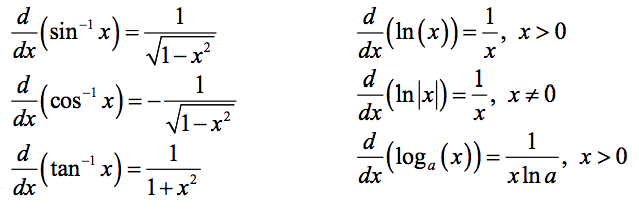
\includegraphics[scale=0.45]{derivatives}

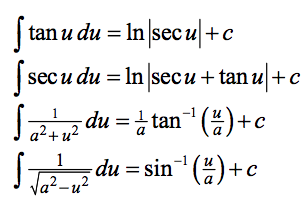
\includegraphics[scale=0.45]{integrals}

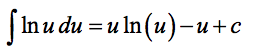
\includegraphics[scale=0.45]{integral_ln}

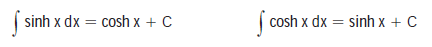
\includegraphics[scale=0.65]{integrals2}

% Matrix Differentiation
\subsection{Matrix Differentiation}

Recommended resource: ``Matrix Differentiation ( and some other stuff )" by Randal J. Barnes (Department of Civil Engineering, University of Minnesota). Available for download at \url{https://atmos.washington.edu/~dennis/MatrixCalculus.pdf}.

More information not contained in that pdf (from the appendix of \textit{Convex Optimization} by Stephen Boyd and Lieven Vandenberghe, available for free download at \url{https://web.stanford.edu/~boyd/cvxbook/}):

\textbf{Chain rule.} Suppose \(f: \mathbb{R}^n \to \mathbb{R}^m\) is differentiable at \(x \in \textbf{int} \textbf{ dom} f\) and  \(g: \mathbb{R}^m \to \mathbb{R}^p\) is differentiable at \(f(x) \in \textbf{int} \textbf{ dom } g\). Define the composition \(h: \mathbb{R}^n \to \mathbb{R}^p\) by \(h(z) =  g(f(x))\). Then

\[
D h(x) = Dg(f(x)) D f(x)
\]

In particular, if \(f: \mathbb{R}^n \to \mathbb{R}\) and  \(g: \mathbb{R} \to \mathbb{R}\),

\[
\nabla h(x) = g'(f(x)) \nabla f(x)
\]

\textbf{Example with an affine function.} Suppose \(f: \mathbb{R}^n \to \mathbb{R}^m\) is differentiable, \(A \in \mathbb{R}^{n \times p}\), and \(b \in \mathbb{R}^n\). Define \(g: \mathbb{R}^p \to \mathbb{R}^m\) as \(g(x) = f(Ax + b)\) with \(\textbf{dom } g = \{x \mid Ax + b \in \textbf{ dom } f \}\). Then 

\[
\nabla g(x) = A^T \nabla f(Ax + b)
\]

\textbf{Example 2.} Consider \(f: \mathbb{R}^n \to \mathbb{R}\) where 

\[
f(x) = \log \sum_{i=1}^m \exp(a_i^Tx + b_i) = 
\]

where \(a_1, \ldots, a_m \in \mathbb{R}^n\)  and \(b_1, \ldots, b_m \in \mathbb{R}\). Note that \(f(\cdot)\) can be expressed as a composition of \(Ax + b\) (where \(A \in \mathbb{R}^{m \times n}\) has rows \(a_1^T , \ldots, a_m^T\)) and the function \(g: \mathbb{R}^m \to \mathbb{R}\) given by \(g(y) = \log( \sum_{i=1}^m \exp(y_i)\). We have

\[
\nabla g(y) = \bigg[ \sum_{i=1}^m e^{y_i} \bigg]^{-1} \big( \exp(y_1) \ldots \exp(y_m) \big) ^T
\]

so applying the chain rule yields

\[
\nabla f(x) =  \bigg[ \sum_{i=1}^m \exp( a_i^T x + b_i) \bigg]^{-1} A^T z
\]

where \(z_i = \exp(a_i^T x + b_i), \ i =1 , \ldots, m\).

\textbf{Hessians.} The Hessian matrix of \(f: \mathbb{R}^n \to \mathbb{R}\) is denoted by \(\nabla^2f(x)\) and is given by

\[
\nabla^2 f(x)_{ij} = \frac{\partial^2 f(x)}{\partial x_i \partial x_j} , \ i = 1, 2, \ldots, n, \ \ \ j = 1, 2, \ldots, n
\]

The quadratic function

\[
f(x_0) + \nabla f(x_0)^T (x - x_0) + \frac{1}{2} (x - x_0)^T \nabla^2 f(x_0) (x - x_0)
\]

is called the \textbf{second-order approximation of \(f\) near \(x_0\)}.

\textbf{Chain rule for second derivative.} A chain rule for the second derivative is difficult in general. Here are some special cases.

\textbf{Composition with scalar function.} Suppose \(f: \mathbb{R}^n \to \mathbb{R}\), \(g: \mathbb{R} \to \mathbb{R}\), and \(h(x) = g(f(x))\). We have

\[
\nabla^2 h(x) = g'(f(x)) \nabla^2 f(x) + g''(f(x)) \nabla f(x) \nabla f(x)^T
\]

\textbf{Composition with affine function.} Suppose  \(f: \mathbb{R} \to \mathbb{R}\), \(a \in \mathbb{R}^m\), \(b \in \mathbb{R}\). Define \(g: \mathbb{R}^m \to \mathbb{R}\) by \(g(x) = f(a^Tx + b)\). Then

\[
\nabla^2 g(x) = a^T \nabla^2 f(a^Tx + b) a
\]


More generally, suppose  \(f: \mathbb{R}^n \to \mathbb{R}\), \(A \in \mathbb{R}^{n \times m}\), and \(b \in \mathbb{R}^n\). Define \(g: \mathbb{R}^m \to \mathbb{R}\) by \(g(x) = f(Ax + b)\). Then

\[
\nabla^2 g(x) = A^T \nabla^2 f(Ax + b) A
\]

% Some theorems in higher dimensions
\subsection{Some theorems in higher dimensions}

\begin{proposition}[\textbf{Change of Variables}]If \(U\) is a ``nice" subset of \(\mathbb{R}^2\) and \(\phi\) is an injective differentiable function on \(U\), then 

\[
 \int_{\phi(U)} f(u,v) dudv = \int_U f(\phi(x,y)) | J \phi(x,y) | dx dy
\]

where \( J \phi(x,y)\) is the Jacobian of \(\phi\) at \((x,y)\).

\end{proposition}

\textbf{Taylor's Theorem (first order).} (borrowed from \url{https://www.rose-hulman.edu/~bryan/lottamath/mtaylor.pdf}) Consider a function \(f: \mathbb{R}^n \to \mathbb{R}\). Let \(a \in \mathbb{R}^n\) be a fixed point. Then Taylor's Theorem states:

\textit{If \(f(x)\) is differentiable on an open ball \(B\) around \(a\) and \(x \in B\) then}

\[
f(x) = f(a) + \nabla f(b)^T(x - a)
\]

\textit{for some \(b\) on the line segment joining \(a\) and \(x\).} 

This can also be expressed as follows. \textit{Let \(x, y \in \mathbb{R}^n\). If \(f(x)\) is continuously differentiable, then}

\[
f(y) = f(x) + \nabla f(tx + (1-t)y)^T  (y - x)
\]

\textit{for some \(t \in [0, 1]\).} 

\begin{proof}
Consider \(g(z) = f(zy + (1-z)x)\). If \(f\) is differentiable then so is \(g\). Then by the Mean Value Theorem, for some \(t \in (0, 1)\) we have \(g(1) - g(0) = g'(t)\). By the chain rule,

\[
g'(t) = \nabla f(x + t(y - x))^T (y - x)
\]

Using \(g(1) = f(y)\) and \(g(0) = f(x)\), we have

\[
\iff  \nabla f(tx + (1-t)y)^T (y - x) = g(1) - g(0) = f(y) - f(x)
\]
\end{proof}

\textbf{Taylor's Theorem (second order).} Consider a function \(f: \mathbb{R}^n \to \mathbb{R}\). Let \(a \in \mathbb{R}^n\) be a fixed point. Then Taylor's Theorem states:

\textit{If \(f(x)\) is twice differentiable on an open ball \(B\) around \(a\) and \(x \in B\) then}

\[
f(x) = f(a) + (x -a)^T \nabla f(a) + \frac{1}{2}(x-a)^T \nabla^2 f(b) (x-a)
\]

\textit{for some \(b\) on the line segment joining \(a\) and \(x\).} 

This can also be expressed as follows. \textit{Let \(x, y \in \mathbb{R}^n\). If \(f(x)\) is twice continuously differentiable, then}

\[
f(y) = f(x) +  \nabla f(x)^T (y -x) + \frac{1}{2}(y - x)^T \nabla^2 f(ty + (1-t)x) (y - x)
\]

\textit{for some \(t \in [0, 1]\).} 

\begin{proof}
Consider \(g(z) = f(zy + (1-z)x)\). If \(f\) is differentiable then so is \(g\). Then by the second order case of Taylor's Theorem in one dimension, for some \(t \in (0, 1)\) we have \(g(1) =  g(0) + g'(0) + (1/2)g''(t)\). By the chain rule,

\[
g''(t) =  \pderiv{}{t} \nabla f(x + t(y - x))^T (y - x) = (y - x)^T \nabla^2 f(x + t(y - x))^T (y - x) 
\]

Using this result along with \(g(1) = f(y)\),  \(g(0) = f(x)\), and \(g'(0) = \nabla f(x)^T (y - x) \),  we have

\[
f(y) = f(x) + \nabla f(x)^T (y - x)  + \frac{1}{2} (y - x)^T \nabla^2 f(x + t(y - x))^T (y - x) 
\]
\end{proof}

% Optimizing functions of several variables
\subsection{Optimizing functions of several variables}

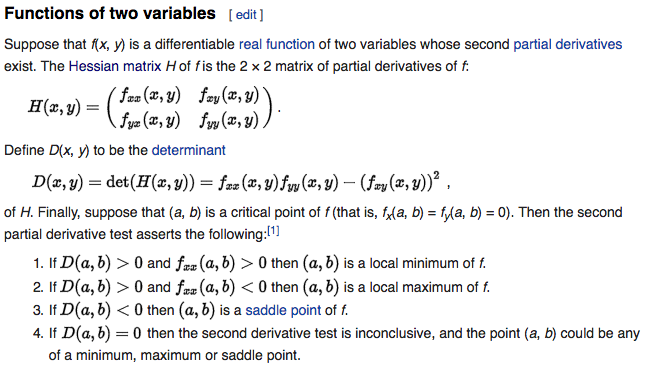
\includegraphics[scale=0.65]{hessian1}

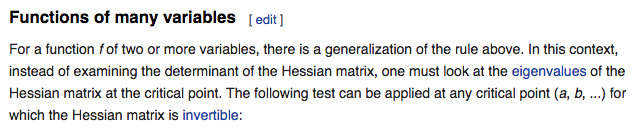
\includegraphics[scale=0.65]{hessian2}

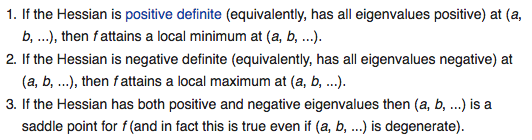
\includegraphics[scale=0.65]{hessian3}

% Lagrange Multipliers
\subsection{Lagrange Multipliers} \textbf{: to flesh out!} http://tutorial.math.lamar.edu/Classes/CalcIII/LagrangeMultipliers.aspx

% Line Integrals
\subsection{Line Integrals} (p. 555 of Strang book)

Suppose a force in two-dimensional space is given by \(\boldsymbol{F} = M\boldsymbol{i} + N \boldsymbol{j}\). Then the work done by this force on a particle moving along a curve \(C\) is given by

\[
W = \int_C \boldsymbol{F} \cdot \text{d}\boldsymbol{R} = \int_C M \text{d}x + N \text{d} y
\]

Along a curve in three-dimensional space the work done by a three-dimensional force \(\boldsymbol{F} = M\boldsymbol{i} + N \boldsymbol{j} + P \boldsymbol{j}\) is given by

\[
W = \int_C \boldsymbol{F} \cdot \boldsymbol{T} \text{d}s = \int_C \boldsymbol{F} \cdot \text{d}\boldsymbol{R} = \int_C M \text{d}x + N \text{d}y + P \text{d}z
\]

where the tangent vector \(\boldsymbol{T}\) is given by \[\boldsymbol{T} = \frac{\text{d}\boldsymbol{R}}{\text{d}s}\]

\textbf{Green's Theorem:} Suppose the region \(R\) is bounded by the simple closed piecewise smooth curve \(C\). Then an integral over \(R\) equals a line integral around \(C\):

\[
\oint_C \boldsymbol{F} \cdot \text{d}\boldsymbol{R} = \oint_C M \text{d}x + N \text{d}y = \int \int_R \bigg( \frac{\partial N}{\partial x} - \frac{\partial M}{\partial y} \bigg) \text{d}x \ \text{d}y
\]

\textbf{Line integrals chapter!} http://tutorial.math.lamar.edu/Classes/CalcIII/LineIntegralsIntro.aspx

\textbf{Surface inegrals chapter!} http://tutorial.math.lamar.edu/Classes/CalcIII/SurfaceIntegralsIntro.aspx

% Miscellaneous
\subsection{Miscellaneous}

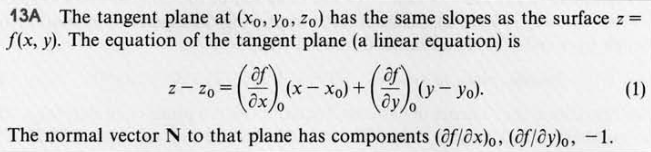
\includegraphics[scale=0.65]{tangent_plane}

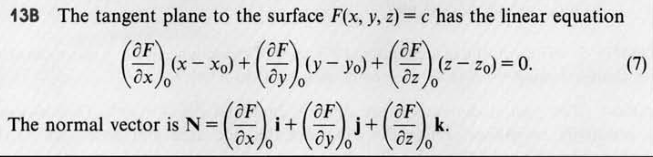
\includegraphics[scale=0.65]{tangent_plane2}

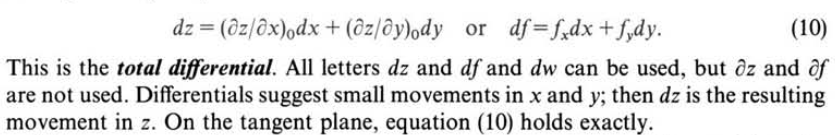
\includegraphics[scale=0.55]{total_differential}

The \textbf{directional derivative}, denoted \(D_v f(x, y)\), is a derivative of a multivariable function in the direction of a vector \(\boldsymbol{v}\). It is the scalar projection of the gradient onto \(\boldsymbol{v}\).

\[
D_v f(x, y) = \text{comp}_v \nabla f(x, y) = \frac{\nabla f(x, y) \cdot \boldsymbol{v}}{|\boldsymbol{v}|}
\]

% Practice Problems
\subsection{Practice Problems}

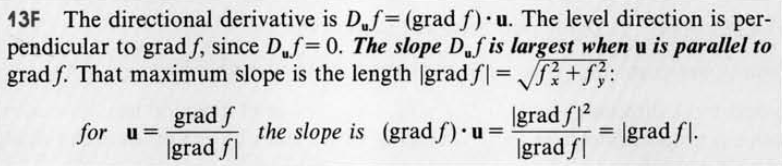
\includegraphics[scale=0.55]{gradient}

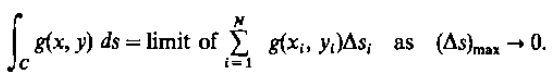
\includegraphics[scale=0.55]{line_int1}

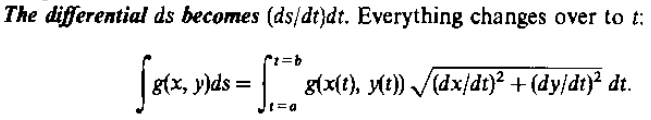
\includegraphics[scale=0.55]{line_int2}

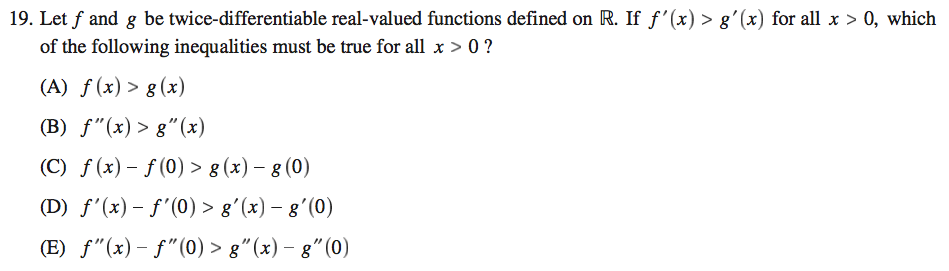
\includegraphics[scale=0.5]{0568_19}

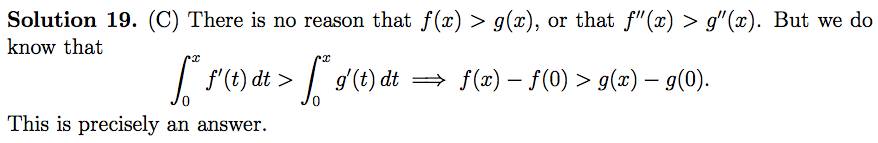
\includegraphics[scale=0.5]{0568_19s}

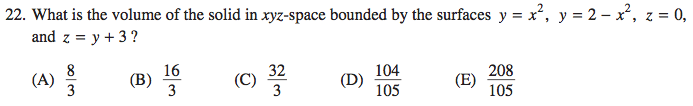
\includegraphics[scale=0.65]{1268_22}

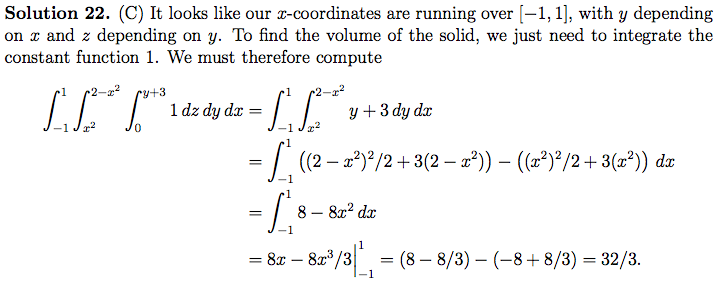
\includegraphics[scale=0.65]{1268_22s}

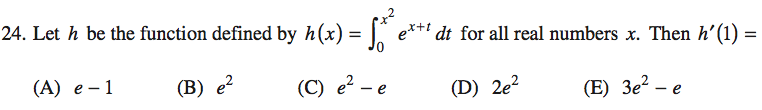
\includegraphics[scale=0.5]{0568_24}

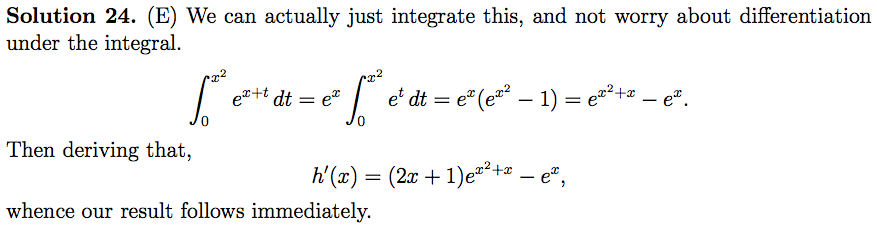
\includegraphics[scale=0.5]{0568_24s}

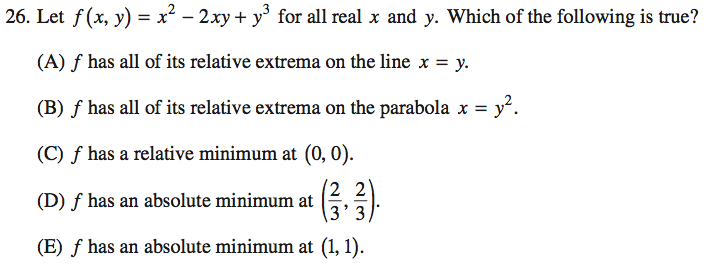
\includegraphics[scale=0.5]{0568_26}

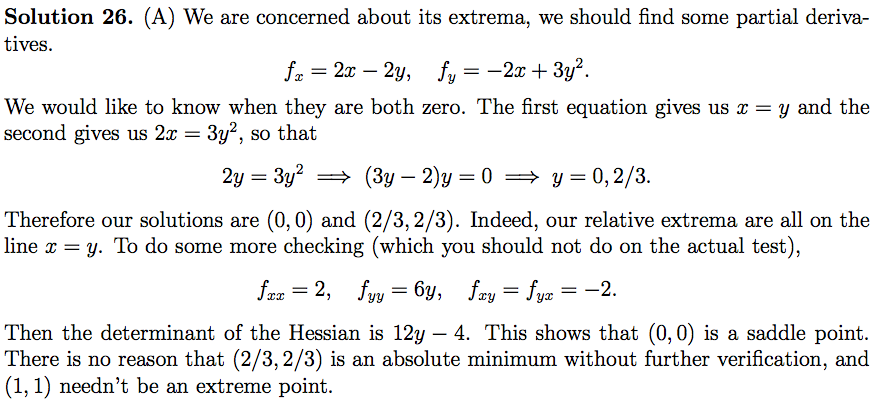
\includegraphics[scale=0.5]{0568_26s}

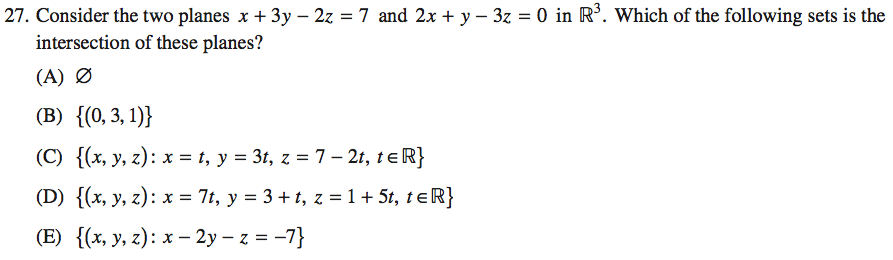
\includegraphics[scale=0.5]{0568_27}

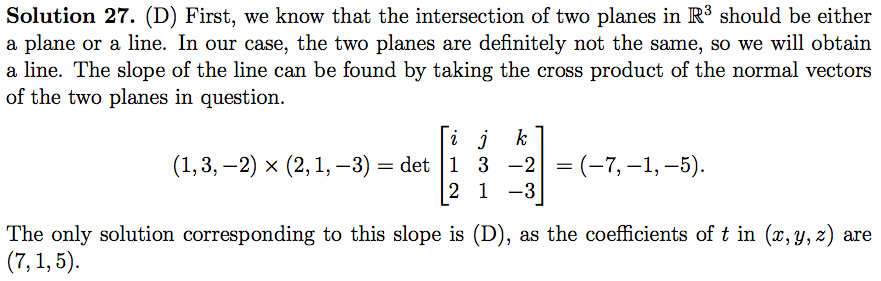
\includegraphics[scale=0.5]{0568_27s}

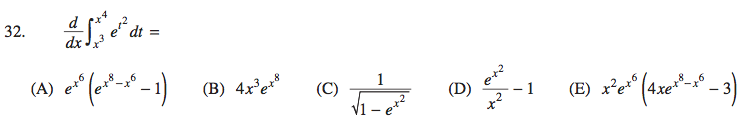
\includegraphics[scale=0.65]{1268_32}

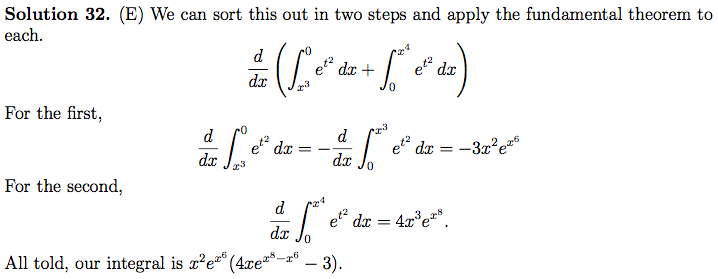
\includegraphics[scale=0.65]{1268_32s}

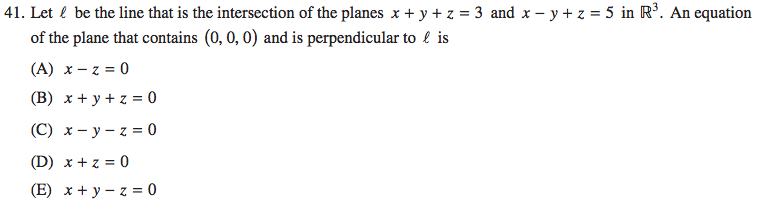
\includegraphics[scale=0.65]{1268_41}

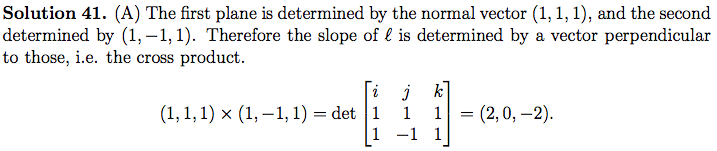
\includegraphics[scale=0.65]{1268_41s1}

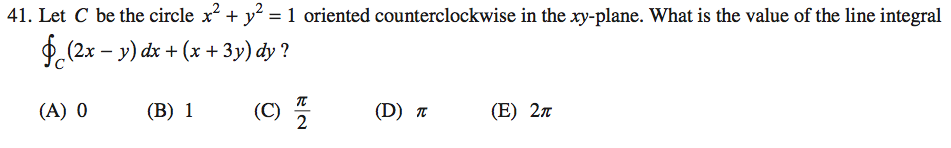
\includegraphics[scale=0.5]{0568_41}

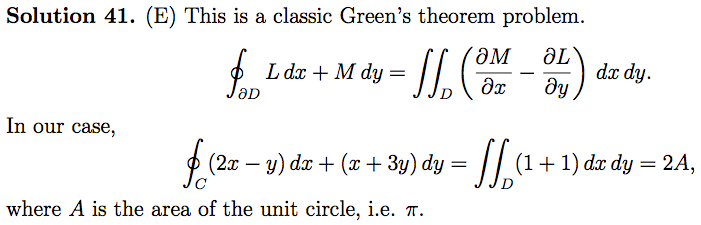
\includegraphics[scale=0.5]{0568_41s}

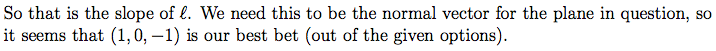
\includegraphics[scale=0.65]{1268_41s2}

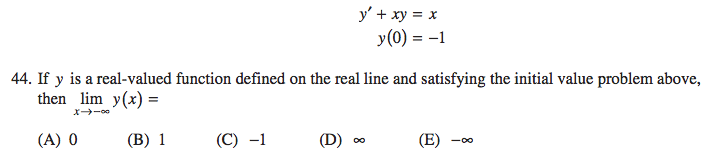
\includegraphics[scale=0.65]{1268_44}

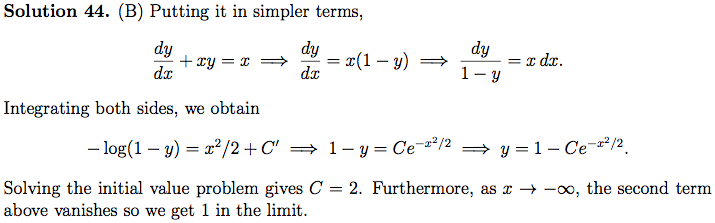
\includegraphics[scale=0.65]{1268_44s}


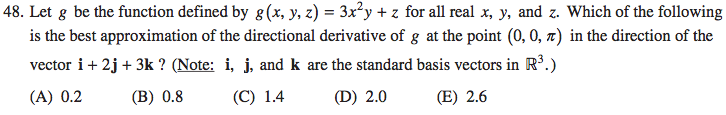
\includegraphics[scale=0.65]{1268_48}

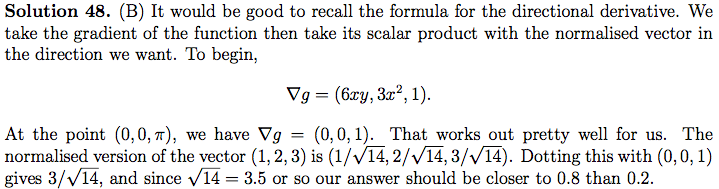
\includegraphics[scale=0.65]{1268_48s}

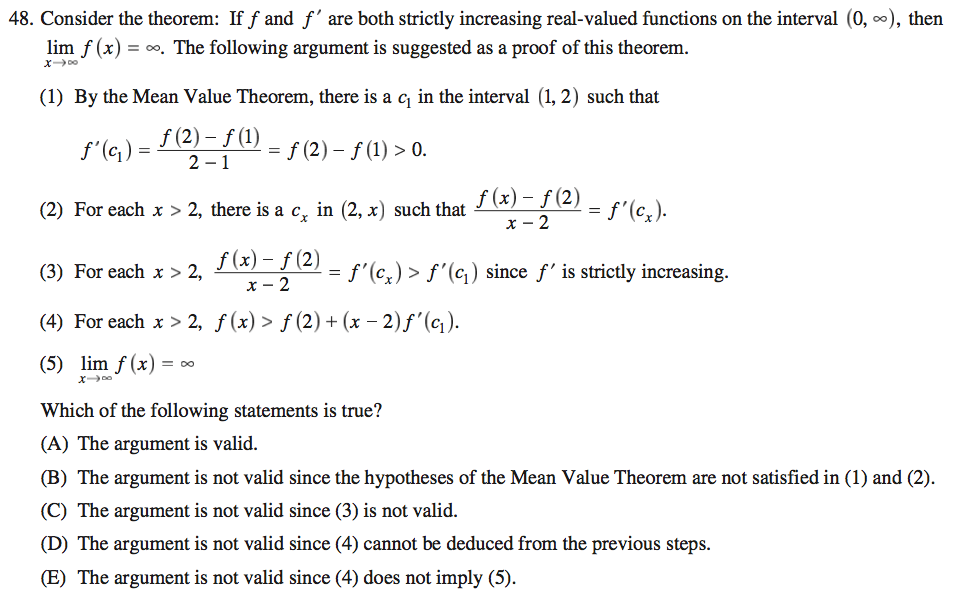
\includegraphics[scale=0.5]{0568_48}

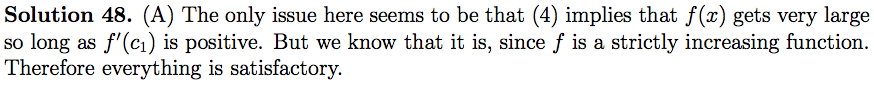
\includegraphics[scale=0.5]{0568_48s}

%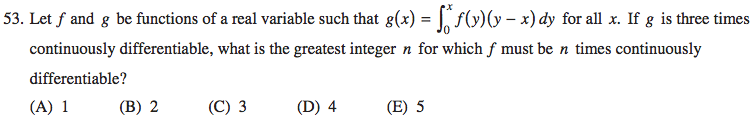
\includegraphics[scale=0.65]{1268_53}

%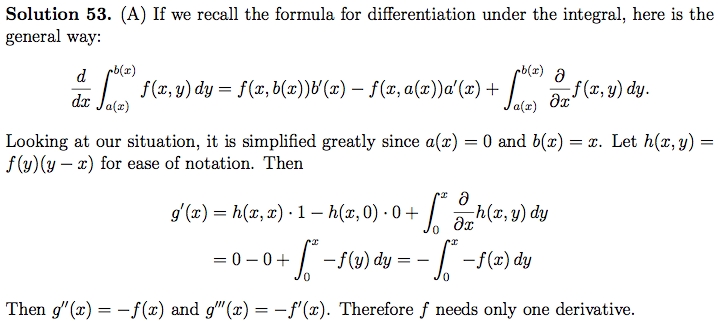
\includegraphics[scale=0.65]{1268_53s}

%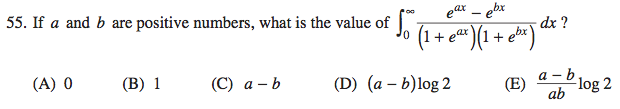
\includegraphics[scale=0.65]{1268_55}

%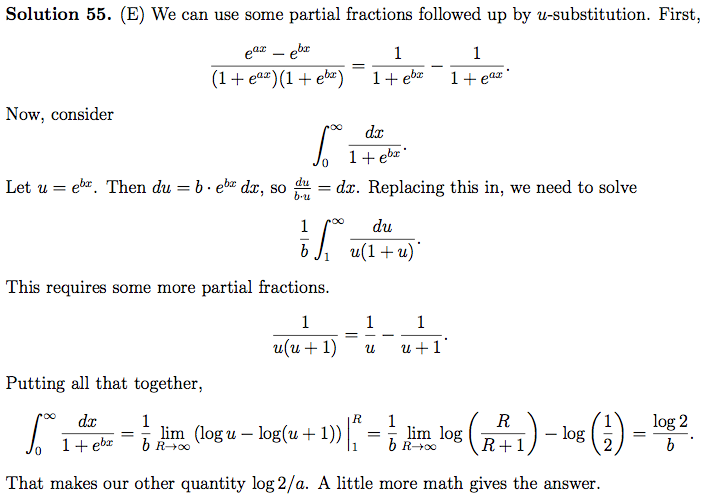
\includegraphics[scale=0.65]{1268_55s}

%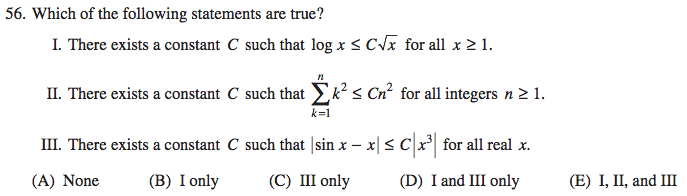
\includegraphics[scale=0.65]{1268_56}
%
%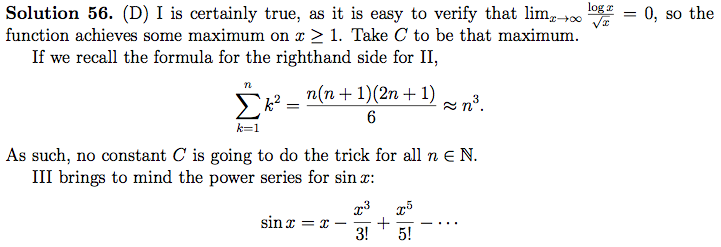
\includegraphics[scale=0.65]{1268_56s1}

%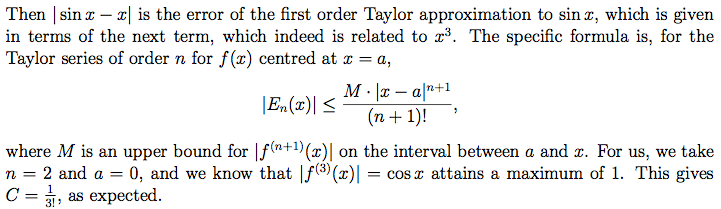
\includegraphics[scale=0.65]{1268_56s2}

%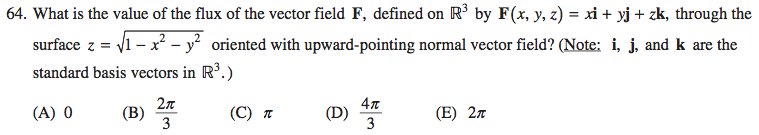
\includegraphics[scale=0.65]{1268_64}
%
%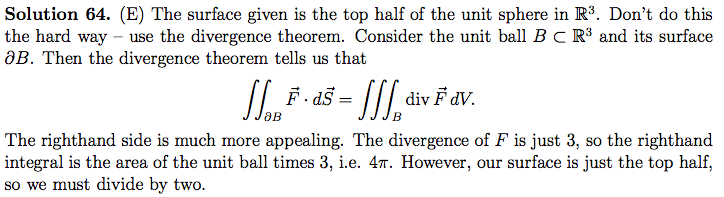
\includegraphics[scale=0.65]{1268_64s}

% 
%
%
%
%
%
%\end{document}